In this chapter, test and evaluation of the system will be described. More specifically, the client-server communication, regression models, and routes are tested and evaluated. The results are held against the solution criteria in section \ref{chap:solutioncriteria}.

\section{Test and evaluation of client-server communication}
To be certain that our client server communication works as it should according to our solution criteria, we will do both "real-life" practical tests and black-box testing, e.g. making sure the client and server behaves as it should on different occasions.

\subsection{Connection between client and server}
To make sure the client(s) can connect to the server we have made these tests. The reasons behind these test is to make sure we have met criterion \ref{crit:severalconnections}. We first check if the server can handle one client and thereafter handle several clients where the clients request the same route. 
\begin{itemize}
	\item From local host, we started the server and afterwards we started the client and connected to the server. We could see that the server accepted the connection.
	\item We downloaded the application to five smartphones and connected to the server, which the server handled correctly. As mentioned in \autoref{chap:clientserver} we requested a route with 2 specific note id's, which gave us a route, we requested the same route on each smartphone and all of the smartphones received the same route. The time we had to wait for all of the smartphones to get the routes was between 5-10 seconds, which is acceptable, but performance has not been a concern in this project.
\end{itemize}

\subsection{Message received matches the message sent}
To be certain the longitude, latitude and speed that is sent is received correctly on the server, which is our solution criteria \ref{crit:sendmessages}, since that data is something that can be used as live data and stored as historical data. We did the following test:
\begin{itemize}
	\item We gave an Android emulator a specific longitude and latitude and then used the application to send the data to the server. We got the following information displayed in \figref{fig:datasentfromclienttoserver}. Which confirms that the message sent from the client is received correctly on the server.
	\begin{figure}[h!]
  \centering
    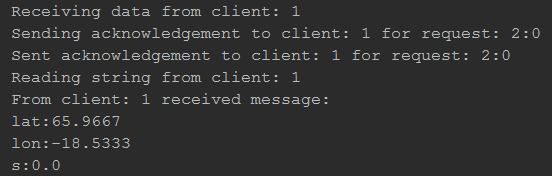
\includegraphics[width=0.8\textwidth]{figures/datasentfromclienttoserver.png}
    \caption{Data received on the server from the client}
    \label{fig:datasentfromclienttoserver}
\end{figure}
\end{itemize}

%\subsection{If a message is lost}
%To be sure that if some message is lost or connection between the client and server is not stable, which we also described in \autoref{chap:clientserver}, we are sending acknowledgements between client server. As  \figref{fig:datasentfromclienttoserver} illustrates when the server receives data from the client the server responds with an acknowledgement message to the client, that it has received the data.

\subsection{Lack of connection}
The user of the application has to be notified if they cant receive or send their data to the server. This is handled by giving a pop-up message to the user of the application that there is no connection to the server.

\subsection{GPS location and speed}
We have to be certain that the data we send is the real data, e.g. get the correct location of the client and get the correct speed, because if this data is not correct we will get false and incorrect data. Besides that if this data is not correct we can not meet solution criterion \ref{crit:sendmessages}. This was tested in the following way.
One person was driving the car and another person was checking the client on a smartphone, where the smartphone displayed the current speed and the location after a click on a button. The speed was compared to the car's speedometer which matched and the GPS location that was shown was later checked on a map, where the locations given by the smartphone also were correct.
\\

